% ! TeX root = distributed-systems-final-report.tex
\section{User Guide}\label{user-guide}

\begin{figure}
    \centering
    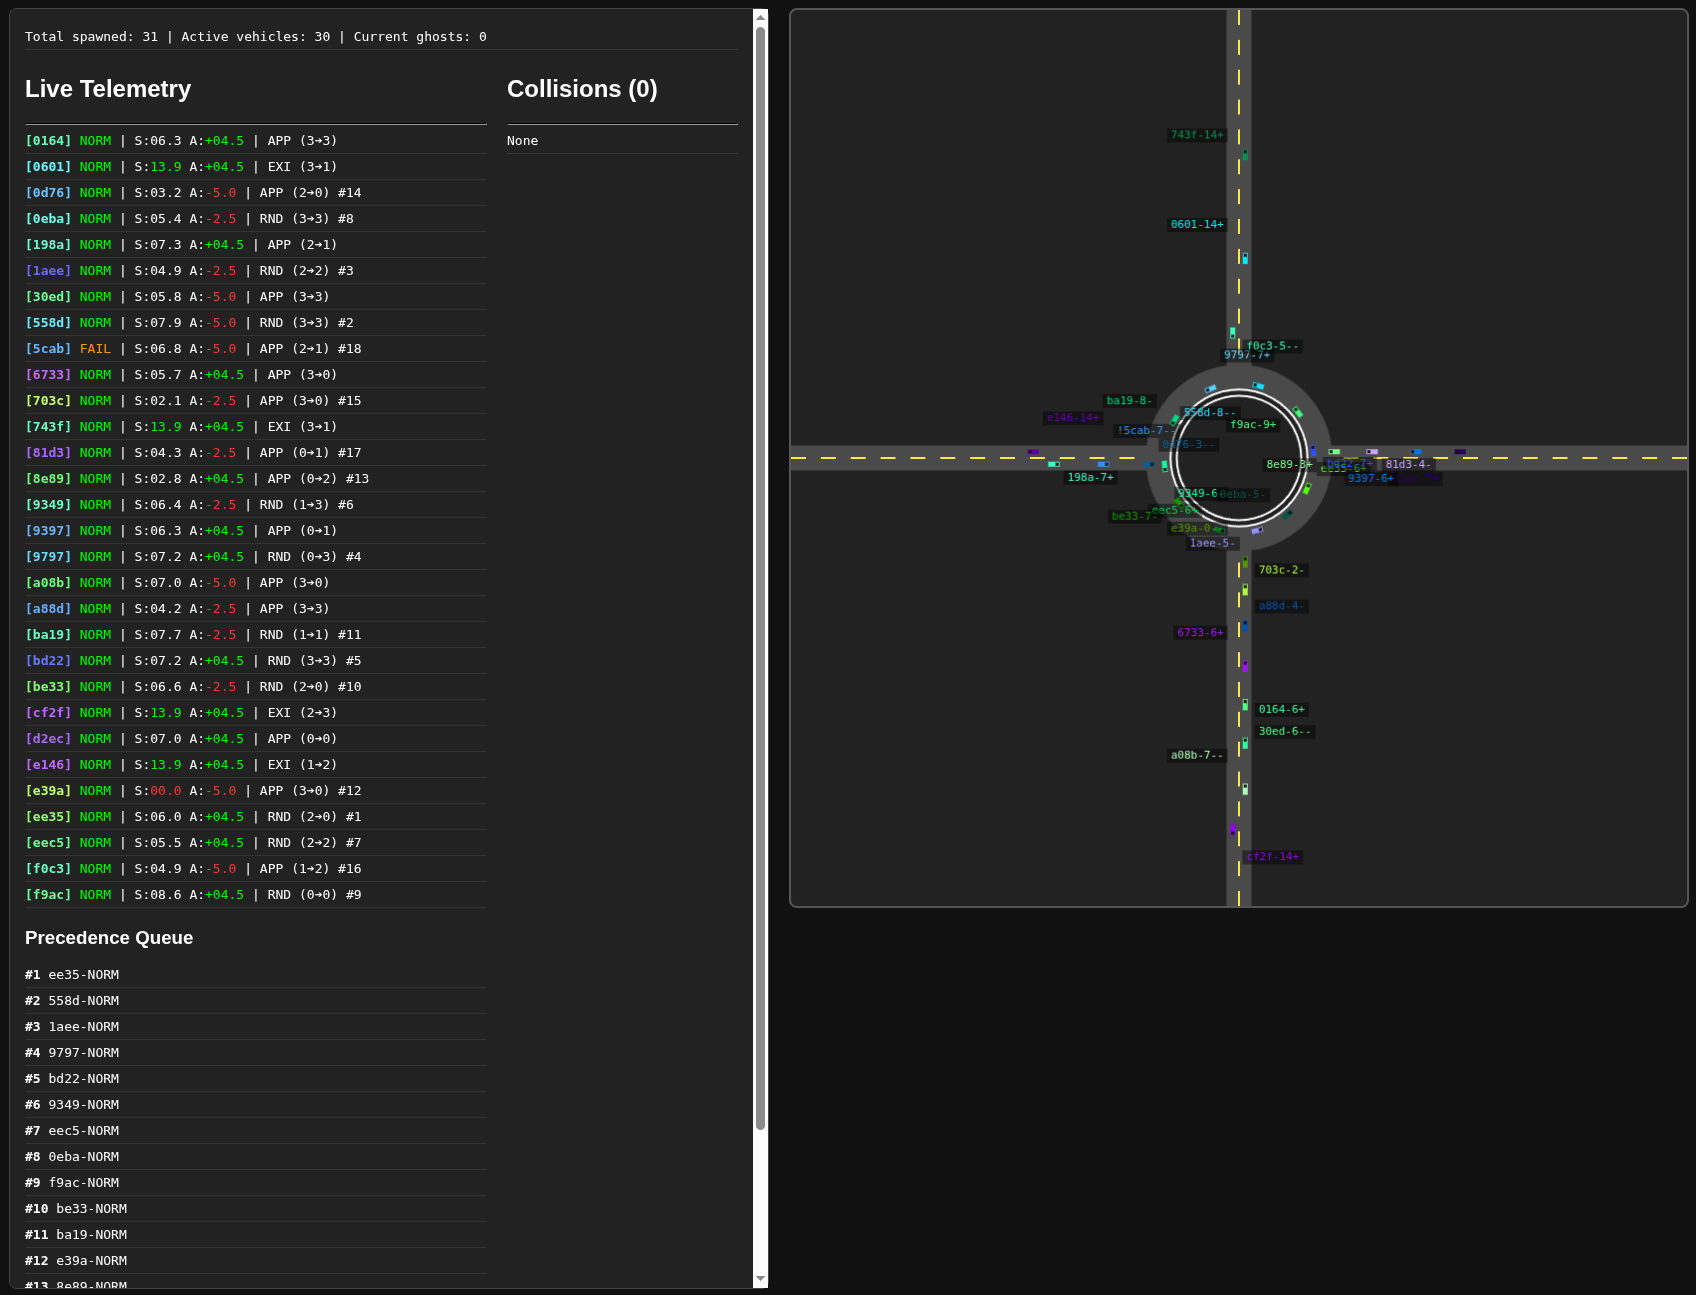
\includegraphics[width=\textwidth]{figures/roundabout-app-screenshot.png}
    \caption{Screenshot of the running web page.}
    \label{fig:class-diagram}
\end{figure}

After the docker compose infrastructure has been deployed successfully, the
simulation can be visualized, from a browser, on the \textbf{page}
\textit{http://localhost:8080}. Cars should be seen moving, proceeding
endlessly.
\\
\\
A \textbf{dashboard} on the left of the page displays:
\begin{itemize}
  \item in the first row, in order, the total number of spawned vehicles in the
  simulation, the current number of vehicles, the current number of ghosts
  identified by the controller;
  \item on the left, a list with each vehicle's telemetry, sorted alphabetically
  by their id. For each vehicle, its row contains, in order: the id's first 4
  characters; a shortened word for its status (normal, failsafe or
  disconnected); speed ``S'' and acceleration ``A''; a shortened word for its
  navigation status (``APP'' for approaching, ``RND'' for in-roundabout, ``EXI''
  for exiting); start and destination road indexes (start number \textit{->} end
  number); position in the priority queue, if present in it;
  \item below the telemetry, the controller's precedence queue, showing the
  vehicles with highest priority on the top;
  \item on the right, the identified collisions. Each one shows: a timestamp
  (\textit{hours:minutes:seconds}), conflicting vehicles ($v_1-v_2$),
  conflicting vehicles' navigation statuses.
\end{itemize}

The actual \textbf{simulation} is shown in the area at the center of the page.
Each vehicle is represented with a random color and a label in a random position
around it; both the label and the id in the dashboard appear of the same colour.
The car's front is represented by its windshield.

\textbf{Ghosts}, as identified by the controller, also appear as grey cars. If a
ghost is displayed over a real vehicle, it means that the controller hasn't been
able to merge them; most likely, this is the expected behaviour: it may mean
that the vehicle is disconnected but the controller has successfully created a
corresponding ghost in its place.

Pressing the \textit{spacebar} will pause or resume the simulation.
\\
\\
The web server also exposes some http endpoints for interacting.

The bash script \textit{src/ctrl.sh} can be used directly. It expects one
command, optionally followed by the vehicles to address:
\begin{itemize}
  \item without specified vehicles, the command is addressed to everyone (e.g.
useful for pausing or resuming);
  \item if it's a number \textit{N} of one or two digits, \textit{N} random
vehicles will be addressed;
  \item otherwise, a string (different from the previously described \textit{N})
  will be used as prefix of a vehicle id and the single vehicle will be
  addressed, if found and unique.
\end{itemize}

Commands can be written as entire words or by their short letter, uppercase or
lowercase:
\begin{itemize}
  \item \textit{pause} (\textit{p})
  \item \textit{resume} (\textit{r})
  \item \textit{failsafe} (\textit{f}): forcefully set to failsafe
  \item \textit{controller} (\textit{c}): undo failsafe (set to normal)
  \item \textit{disconnect} (\textit{d}): forcefully set to disconnected
  \item \textit{reconnect} (\textit{n}): undo disconnect (set to normal, like
  for \textit{c})
\end{itemize}

Examples:
\begin{verbatim}
# Usage: src/ctrl.sh {PAUSE|RESUME|FAILSAFE|CONTROLLER|DISCONNECT|RECONNECT}
#                    [vehicle-id|vehicle-count]
#     or src/ctrl.sh {p|r|f|c|d|n} [vehicle-id|vehicle-count]

# pause/resume simulation
./src/ctrl.sh p
./src/ctrl.sh r
./src/ctrl.sh resume
# enter failsafe
./src/ctrl.sh f
# exit failsafe, for vehicle with ID starting with 4fd2
./src/ctrl.sh c 4fd2
# mark 10 random vehicles as disconnected
./src/ctrl.sh d 10
# exit disconnected
./src/ctrl.sh n
\end{verbatim}

These commands can be used to inject some chaos in the simulation and see how
the vehicles behave; pausing also allows to analyze better the situation and,
for example, to pick a precise vehicle, change its status and see if this will
cause an accident.
\\
\\
The corresponding http API endpoints are:
\begin{itemize}
    \item \textbf{GET /api/config}: retrieves the static geometrical
    configuration of the simulated roundabout. Returns a JSON object containing
    physical constants such as \texttt{r\_radius}, \texttt{lane\_width}, and
    \texttt{car\_length}.
    \item \textbf{GET /api/state}: retrieves the current real-time state of the
    distributed system. Returns a JSON object containing the active
    \texttt{vehicles} dictionary, the \texttt{precedence\_queue}, identified
    \texttt{ghosts} (disconnected nodes), and a list of detected
    \texttt{collisions}.
    \item \textbf{POST /api/control}: submits a \texttt{SystemCommand} to alter
    the simulation state or inject network faults. Accepts a JSON payload
    requiring a \texttt{command} string (\textit{PAUSE, RESUME, ENTER\_FAILSAFE,
    EXIT\_FAILSAFE,} \textit{ENTER\_DISCONNECTED, EXIT\_DISCONNECTED}).
    Optionally accepts \texttt{vehicle\_id} to target a specific node, or
    \texttt{vehicle\_count} to apply the fault to a random subset of nodes,
    otherwise will target all if left empty.
\end{itemize}
